\dev{Emile Martinez}{}

\textit{Dans cette leçon on déroule un exemple d'utilisation de l'orienté objet, avec la modélisation et l'aspect modulaire, mais également une illustration de ce qui est fonctionnel, impératif, etc...}

\paragraph{Objectif} Représenter une personne voulant se déplacer sur une carte.

\begin{figure}
    \centering
    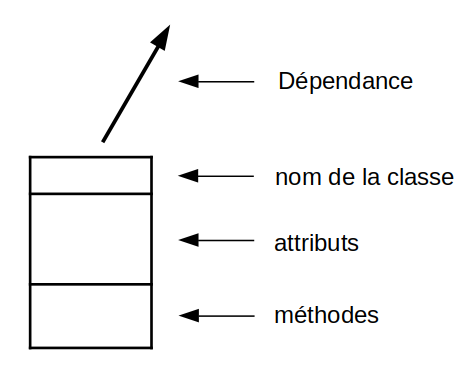
\includegraphics[scale=0.5]{Developpements/Illustration oriente objet/explication uml.png}
    \caption{Explication des champs de notre diagramme}
\end{figure}

\begin{com}
    Construire le diagramme suivant petit à petit, et ne rajouter les éléments seulement quand on en a besoin. (par exemple, la File, ne la rajouter que quand on en aura besoin)
\end{com}

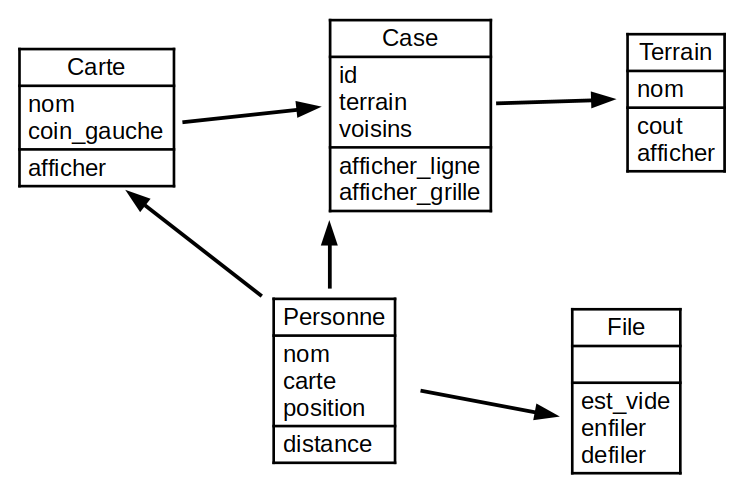
\includegraphics[scale=0.5]{Developpements/Illustration oriente objet/diagramme uml.png}

\begin{figure}
    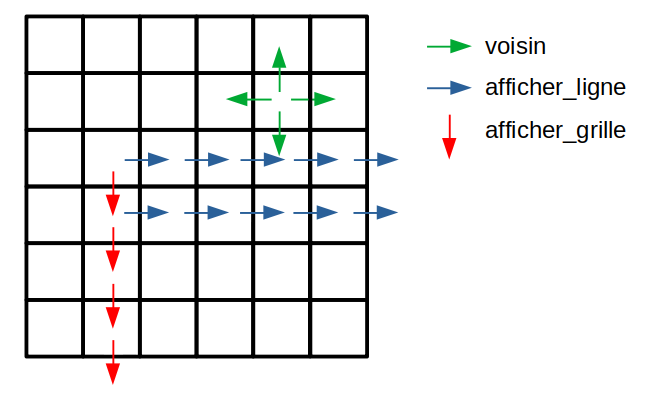
\includegraphics[scale=0.5]{Developpements/Illustration oriente objet/explication carte.png}
    \caption{Explication de la carte et du fonctionnement de afficher}
	\label{carteobj1}
\end{figure}

\begin{lstlisting}
class Carte:
    def __init__(self, ...):
        self.nom = ...
        self.coin_gauche = ...
    
    def afficher(self):
        self.coin_gauche.afficher_grille()    
\end{lstlisting}

\begin{lstlisting}
class Case:
    def __init__(self, ...):
        self.terrain = ...
    self.voisins = ... #dictionnaire de clé "haut", "gauche", etc...
    
    def afficher_ligne(self):
        self.terrain.afficher()
        if "droite" in self.voisins:
            self.voisins["droite"].afficher_ligne()
        else:
            print() # on met une nouvelle ligne
    
    def afficher_grille(self):
        self.afficher_ligne()
        if "bas" in self.voisins:
            self.voisins["bas"].afficher_grille()
\end{lstlisting}

\begin{com}
	Expliquer ici pourquoi on fait un parcours en largeur, en montrant sur la figure \ref{carteobj1} que on peut ainsi trouver un chemin en plus ou moins ligne droite pour y aller	
\end{com}

\begin{com}
	Introduire ici la nécessité d'une structure de file comme il n'en existe pas de natives intéressantes en python, et donc la rajouter au diagramme UML
\end{com}

\begin{lstlisting}
class Personne:
    def __init__(self, ...):
        self.nom = ...
        self.carte = ...
        self.position = ...
    
    def distance(self, dest):
        distance = dict()
        a_voir = File()
        a_voir.ajouter(self)
        distance[self.id] = 0
        while not a_voir.est_vide():
            c = a_voir.defiler()
            if c.id == dest:
                return distance[c.id]
            else:
                for v in c.voisins.values():
                    if v.id not in distance:
                        distance[v] = distance[c] + v.terrain.cout()
                        a_voir.enfiler(v)
        
        return -1
\end{lstlisting}

\begin{com}
	Mentionner ici l'importance de la modularité, puisque on peut alors utiliser file indépendemment de son implémentation.
\end{com}

\begin{com}
	Dire que ici cohabite le fonctionnel et l'impératif, en marquant d'une couleur les lignes récursives (celles où on affiche) et d'une autre l'impératif (l'algo de la distance)
\end{com}

\begin{com}
	Dire pour le jury que là on a écrit au tableau mais que en vrai on le projetterai écrit, et que là on a pas mis beaucoup de commentaires, la spécification, etc..., mais que en vrai évidemment dans le code on le ferait, parce que c'est très important.
\end{com}